\section{Experimental Study}
\label{sec:exp}

Sections~\ref{sec:exp:setup}--\ref{sec:exp:protocols} detail our setup across five evaluation facets:
\ding{172}~end-to-end quality, tokens, and latency on Full and \LIMIT~10 (Section~\ref{sec:exp:e1});
\ding{173}~cost-model surface fidelity and planner regret across $(k,h)$ and header ratios (Section~\ref{sec:exp:e2});
\ding{174}~scalability to $n{=}10{,}000$ (Section~\ref{sec:exp:scale});
\ding{175}~KV prefix caching and discount $\beta$ sensitivity (Section~\ref{sec:exp:cache}); and
\ding{176}~demand adaptation from small \LIMIT~$K$ to Full (Section~\ref{sec:exp:limit-sweep}).

\subsection{Experimental Setup}
\label{sec:exp:setup}

\stitle{Datasets.}
E1 spans 151 queries over six benchmarks (Table~\ref{tab:datasets}): SemBench Movie Q9~\cite{lao2026sembench} (128 reviews of one movie ranked by sentiment against rating grades), plus 30 queries each from TREC DL20~\cite{arxiv21trecdl20}, DL22~\cite{arxiv25trecdl22}, and BEIR~\cite{arxiv21BEIR} (TREC-COVID, DBpedia-Entity, Robust04). For retrieval suites, let $J_q$ count distinct judged candidates with text for query $q$; we select queries with $J_q > 100$ and at least two grades, stratified by pool size and dominant-grade share, sampling $n = \min(J_q, 500)$ proportionally when $J_q > 500$ (collapsing official equivalence classes first on DL22). Outside E1, BM25 pools use three length-stratified queries each from DL20 and TREC-COVID unless noted.

% Corpus sizes are source collection sizes, not per-query E1 input sizes.
% E1 query counts: frozen experiment.yaml and paper-delivery readiness record.
\begin{table}[t]
  \centering\small
  \caption{Source collections and query counts for E1.}
  \label{tab:datasets}
  \setlength{\tabcolsep}{3pt}
  \begin{tabular*}{\columnwidth}{@{\extracolsep{\fill}}llrlr@{}}
    \toprule
    Suite & Dataset & $|D|$ & Domain & Queries \\
    \midrule
    SemBench & Q9 & 1,375,738 & Movie reviews & 1 \\
    \midrule
    \multirow{2}{*}{TREC} & DL20 & 8,841,823 & Web passages & 30 \\
                          & DL22 & 138,364,198 & Web passages & 30 \\
    \midrule
    \multirow{3}{*}{BEIR} & TREC-COVID & 171,332 & Biomedical & 30 \\
                         & DBpedia-Entity & 4,635,922 & Wikipedia & 30 \\
                         & Robust04 & 528,155 & Newswire & 30 \\
    \bottomrule
  \end{tabular*}
\end{table}


\stitle{Baselines and Operators.}
We compare SW and LT($h$) against four OrderByLLM methods (Pointwise, External Pointwise, External Bubble, External Merge)~\cite{DBLP:journals/corr/abs-2509-00303}, ListK Sort and Tournament~\cite{DBLP:journals/corr/abs-2603-17223}, LOTUS Quicksort~\cite{DBLP:journals/pvldb/PatelJPGAGZ25}, and Setwise Heap~\cite{DBLP:conf/sigir/ZhuangZKZ24}. Table~\ref{tab:ranking-algorithms} summarizes logical calls for ten Full and nine \LIMIT~10 methods, omitting ListK Sort under \LIMIT~10 because ListK Select outputs an unordered set.

\stitle{Implementation Details.}
Both Qwen3.5-9B (2-way TP, default $m{=}20$) and Qwen3.8-27B (4-way TP, $m{=}22$ from pilot sweeps)~\cite{DBLP:journals/corr/abs-2505-09388} are served via vLLM~\cite{kwon2023efficient} at temperature zero and seed zero. OrderByLLM and ListK use window size $20$; Setwise Heap compares a parent with two children in one permutation. Full materializes each pass, while \LIMIT~$K$ pulls on demand without prefetching.

% Logical ranker calls, not measured requests or token costs.
\begin{table}[t]
  \centering\small
  \caption{Evaluated semantic ranking operators and logical LLM call complexities for Full and \LIMIT~$K$ execution.}
  \label{tab:ranking-algorithms}
  \setlength{\tabcolsep}{2.6pt}
  \begin{tabular*}{\columnwidth}{@{\extracolsep{\fill}}llcc@{}}
    \toprule
    Method & Prompt & Full & LIMIT $K$ \\
    \midrule
    Pointwise & Point & $n$ & $n$ \\
    Ext.\ Pointwise & Point & $r$ & $r$ \\
    Ext.\ Bubble & List & $O(r^2)$ & $O(r\lceil K/m\rceil)$ \\
    Ext.\ Merge & List & $O(r[1+\log_2 r])$ & $O(r[1+\log_2^+(K/m)])$ \\
    \midrule
    ListK Sort & List & $O(n\log n/\chi_p+n)^{*}$ & Not evaluated \\
    Tournament & List & $C_{\mathrm{tour}}(n)$ & $C_{\mathrm{tour}}(K)$ \\
    \midrule
    LOTUS Quick & Pair & $O(n\log n)^{*}$ & $O(n+K\log K)^{*}$ \\
    Setwise Heap & Set & $O(n\log n)$ & $O(n+K\log n)$ \\
    \midrule
    \SW{} & List & $r+A_{\SW{}}$ & $r+A_{\SW{},K}$ \\
    \LT($h$) & List & $r+A_{\LT{}}$ & $r+A_{\LT{},K}$ \\
    \bottomrule
  \end{tabular*}\par\smallskip
  {\raggedright\footnotesize
  $n$ is the input size, $m$ the batch capacity of the method, and $r=\lceil n/m\rceil$.
  $\log_2^+(x)=\max(0,\log_2 x)$; $\chi_p=(m-p)\log(p+1)$ for $p$ pivots.
  $C_{\mathrm{tour}}(q)$ counts tournament calls until $q$ outputs.
  $A_f$ and $A_{f,K}$ count Full and on-demand merge calls, respectively
  (Section~\ref{sec:cost}). $^{*}$ denotes expected costs under the source pivot models. Counts exclude retries, calibration, and profiling.\par}
\end{table}


\subsection{Experiment-Specific Settings}
\label{sec:exp:protocols}

\stitle{End-to-end ranking (E1).}
Full uses Spearman's $\rho$ (midranks for ties) and \LIMIT~10 uses nDCG@10 (gain $2^g - 1$). Across ten shared input permutations (seeds $0$--$9$), we average quality over queries per dataset and report mean $\pm$ SD across the ten dataset means. Quality/token runs allow ten concurrent queries and count all Input + Output tokens (including Phase~1). Isolated latency uses seed~$0$, one active query, and up to 256 concurrent requests, timing profiling through output return. Token columns sum dataset means for Q9, TREC, and BEIR; latency averages all six datasets equally, and $Q$, $T$, $L$ rank methods by mean within-dataset rank.

\stitle{Cost prediction (E2).}
E2 compares predicted and measured merge input tokens across fixed $(k,h)$ grids on two 500-candidate base workloads: DL20 (query 1109707, 9B) and TREC-COVID (query 38, 27B) under Full and \LIMIT~10. Surface agreement evaluates prediction accuracy; the gap between the planner's pick and the empirical grid minimum measures decision regret. Two padded-instruction workloads on DL20 query 1109707 (Full on 9B, $n{=}641$; \LIMIT~2 on 27B, $n{=}500$) vary fixed header $H$ at fixed item texts $L$.

\stitle{Input size (E3).}
E3 scales $n$ across $1{,}000$, $5{,}000$, and $10{,}000$ on 9B DL20 using nested samples anchored at the BM25 top 1,000, holding five $(k,h)$ pairs per family fixed (Figure~\ref{fig:e3-scale}; four extra LT pairs at larger sizes are omitted from the plot).

\Needspace{5\baselineskip}
\stitle{Prefix caching (E4).}
On 9B, with input tokens $U$, shared-prefix cache hits $Q$, and price factor $\beta \in [0,1]$, equivalent input cost is $C_\beta = U - (1-\beta)Q$ ($U$ when Off; isolated cold namespace per sort when On). E4a compares Off and On-cold ($\beta{=}0$) at $n \in \{100, 500\}$ on medium-length DL20 and COVID queries over eight evenly spaced $(k,h)$ pairs, pooling savings $100(1 - \sum_q C_{0,q}^{\mathrm{On}} / \sum_q U_q^{\mathrm{Off}})$ in Figure~\ref{fig:e4a-c2}. On DL20 ($n{=}500$, LT Full), E4b reprices seven configurations across $\beta \in \{0,.1,.25,.5,.75,.9,1\}$ (five shown in Figure~\ref{fig:e4b-beta}).

\stitle{Output size (E5).}
Across the six BM25 pools at $n{=}500$ on 9B, E5 varies $K$ over $10, 20, 50, 100, 200, 300, 400, 490$, and $500$ alongside Full under Off and On-cold ($\beta{=}0$), selecting $(k,h)$ per demand and cache state to track $C_0$ and nDCG@10 (unjudged gain zero); comparing \LIMIT~500 with Full isolates pass-materialization overhead.

\noindent\textit{Layout review copy.} The results tables and plots contain illustrative values, not experimental measurements.
% E1 through E5: results prose intentionally empty.
% Group the E1/E2 draft assets on one dedicated full-width float page.
\FloatBarrier
\begin{figure*}[p]
  \begingroup
  \renewenvironment{table*}[1][]{%
    \noindent\begin{minipage}{\textwidth}\captionsetup{type=table}\centering
  }{\end{minipage}\par\vskip1pt}%
  \renewenvironment{figure*}[1][]{%
    \noindent\begin{minipage}{\textwidth}\captionsetup{type=figure}\centering
  }{\end{minipage}\par\vskip1pt}%
\subsection{End-to-End Ranking}
\label{sec:exp:e1}
% Synthetic layout preview from round2/tables-pseudocode/src/synthetic.py.
% Single full-width 27-column dual-model table with uncrowded typography & Ours row highlight.
\begin{table*}[t]
\centering
\caption{End-to-end Full ranking quality (Spearman's $\rho\uparrow$), total tokens ($\times 10^{3}\downarrow$), and isolated latency ($\text{s}\downarrow$) across six benchmarks.}
\label{tab:exp1-full}
\begingroup
\normalfont\rmfamily\fontsize{6.4}{8.3}\selectfont
\renewcommand{\qpm}[2]{\mbox{\IfBeginWith{#1}{0.}{\StrGobbleLeft{#1}{1}}{#1}\kern0.35pt{\normalfont\textcolor[HTML]{64748B}{\fontsize{4.8}{5.8}\selectfont\textpm\IfBeginWith{#2}{0.}{\StrGobbleLeft{#2}{1}}{#2}}}}}
\setlength{\tabcolsep}{0pt}
\renewcommand{\arraystretch}{0.96}
\begin{tabular*}{\textwidth}{@{\extracolsep{\fill}}l!{\hspace{2.2pt}}c!{\hspace{1.6pt}}c!{\hspace{1.6pt}}c!{\hspace{1.6pt}}c!{\hspace{1.6pt}}c!{\hspace{1.6pt}}c!{\hspace{2.6pt}}c!{\hspace{1.5pt}}c!{\hspace{1.5pt}}c!{\hspace{2.4pt}}c!{\hspace{2.4pt}}c!{\hspace{1.1pt}}c!{\hspace{1.1pt}}c!{\hspace{3.6pt}\color[HTML]{CBD5E1}\vrule width 0.55pt\hspace{3.6pt}}c!{\hspace{1.6pt}}c!{\hspace{1.6pt}}c!{\hspace{1.6pt}}c!{\hspace{1.6pt}}c!{\hspace{1.6pt}}c!{\hspace{2.6pt}}c!{\hspace{1.5pt}}c!{\hspace{1.5pt}}c!{\hspace{2.4pt}}c!{\hspace{2.4pt}}c!{\hspace{1.1pt}}c!{\hspace{1.1pt}}c@{}}
\toprule
& \multicolumn{13}{c}{\fontsize{7.2}{8.2}\selectfont\textbf{\textcolor[HTML]{1F5A8A}{Qwen3.5-9B}}} & \multicolumn{13}{c}{\fontsize{7.2}{8.2}\selectfont\textbf{\textcolor[HTML]{A63A50}{Qwen3.8-27B}}} \\
\cmidrule(lr){2-14}\cmidrule(lr){15-27}
\textbf{Method} & \multicolumn{6}{c}{Quality $\rho\uparrow$} & \multicolumn{3}{c}{Tokens ($\times 10^{3}$)$\downarrow$} & Lat.$\downarrow$ & \multicolumn{3}{c}{Rank$\downarrow$} & \multicolumn{6}{c}{Quality $\rho\uparrow$} & \multicolumn{3}{c}{Tokens ($\times 10^{3}$)$\downarrow$} & Lat.$\downarrow$ & \multicolumn{3}{c}{Rank$\downarrow$} \\
\cmidrule(lr){2-7}\cmidrule(lr){8-10}\cmidrule(lr){12-14}\cmidrule(lr){15-20}\cmidrule(lr){21-23}\cmidrule(lr){25-27}
& Q9 & DL20 & DL22 & COVID & DBP & R04 & Q9 & TREC & BEIR & s & $Q$ & $T$ & $L$ & Q9 & DL20 & DL22 & COVID & DBP & R04 & Q9 & TREC & BEIR & s & $Q$ & $T$ & $L$ \\
\midrule
Pointwise & \underline{\qpm{0.820}{0.012}} & \underline{\qpm{0.820}{0.012}} & \underline{\qpm{0.820}{0.012}} & \textbf{\qpm{0.840}{0.012}} & \textbf{\qpm{0.840}{0.012}} & \textbf{\qpm{0.840}{0.012}} & \textbf{1.00} & \textbf{2.03} & \textbf{3.12} & \textbf{1.75} & \textbf{1} & \textbf{1} & \textbf{1} & \underline{\qpm{0.840}{0.012}} & \underline{\qpm{0.840}{0.012}} & \underline{\qpm{0.840}{0.012}} & \textbf{\qpm{0.860}{0.012}} & \textbf{\qpm{0.860}{0.012}} & \textbf{\qpm{0.860}{0.012}} & \textbf{5.00} & \textbf{10.03} & \textbf{15.12} & \textbf{2.25} & \textbf{1} & \textbf{1} & \textbf{1} \\
Ext.\ Point. & \textbf{\qpm{0.840}{0.013}} & \textbf{\qpm{0.840}{0.013}} & \textbf{\qpm{0.840}{0.013}} & \underline{\qpm{0.820}{0.013}} & \underline{\qpm{0.820}{0.013}} & \qpm{0.800}{0.013} & \underline{1.10} & \underline{2.23} & \underline{3.42} & \underline{2.15} & \underline{2} & \underline{2} & \underline{2} & \textbf{\qpm{0.860}{0.013}} & \textbf{\qpm{0.860}{0.013}} & \textbf{\qpm{0.860}{0.013}} & \underline{\qpm{0.840}{0.013}} & \underline{\qpm{0.840}{0.013}} & \qpm{0.820}{0.013} & \underline{5.10} & \underline{10.23} & \underline{15.42} & \underline{2.65} & \underline{2} & \underline{2} & \underline{2} \\
Ext.\ Bubble & \qpm{0.800}{0.014} & \qpm{0.800}{0.014} & \qpm{0.800}{0.014} & \qpm{0.800}{0.014} & \qpm{0.780}{0.014} & \underline{\qpm{0.820}{0.014}} & 1.20 & 2.43 & 3.72 & 2.55 & 3 & 3 & 3 & \qpm{0.820}{0.014} & \qpm{0.820}{0.014} & \qpm{0.820}{0.014} & \qpm{0.820}{0.014} & \qpm{0.800}{0.014} & \underline{\qpm{0.840}{0.014}} & 5.20 & 10.43 & 15.72 & 3.05 & 3 & 3 & 3 \\
Ext.\ Merge & \qpm{0.780}{0.015} & \qpm{0.780}{0.015} & \qpm{0.780}{0.015} & \qpm{0.780}{0.015} & \qpm{0.800}{0.015} & \qpm{0.780}{0.015} & 1.30 & 2.63 & 4.02 & 2.95 & 4 & 4 & 4 & \qpm{0.800}{0.015} & \qpm{0.800}{0.015} & \qpm{0.800}{0.015} & \qpm{0.800}{0.015} & \qpm{0.820}{0.015} & \qpm{0.800}{0.015} & 5.30 & 10.63 & 16.02 & 3.45 & 4 & 4 & 4 \\
\midrule
ListK Sort & \qpm{0.760}{0.016} & \qpm{0.760}{0.016} & \qpm{0.760}{0.016} & \qpm{0.760}{0.016} & \qpm{0.760}{0.016} & \qpm{0.760}{0.016} & 1.40 & 3.10 & 6.00 & 3.35 & 5 & 6 & 5 & \qpm{0.780}{0.016} & \qpm{0.780}{0.016} & \qpm{0.780}{0.016} & \qpm{0.780}{0.016} & \qpm{0.780}{0.016} & \qpm{0.780}{0.016} & 5.40 & 11.10 & 18.00 & 3.85 & 5 & 6 & 5 \\
Tournament & \qpm{0.740}{0.017} & \qpm{0.740}{0.017} & \qpm{0.740}{0.017} & \qpm{0.740}{0.017} & \qpm{0.740}{0.017} & \qpm{0.740}{0.017} & 1.41 & 3.12 & 5.10 & 3.75 & 6 & 5 & 6 & \qpm{0.760}{0.017} & \qpm{0.760}{0.017} & \qpm{0.760}{0.017} & \qpm{0.760}{0.017} & \qpm{0.760}{0.017} & \qpm{0.760}{0.017} & 5.41 & 11.12 & 17.10 & 4.25 & 6 & 5 & 6 \\
\midrule
LOTUS Quick & \qpm{0.720}{0.018} & \qpm{0.720}{0.018} & \qpm{0.720}{0.018} & \qpm{0.720}{0.018} & \qpm{0.720}{0.018} & \qpm{0.720}{0.018} & 3.00 & 6.03 & 9.12 & 4.15 & 7 & 7 & 7 & \qpm{0.740}{0.018} & \qpm{0.740}{0.018} & \qpm{0.740}{0.018} & \qpm{0.740}{0.018} & \qpm{0.740}{0.018} & \qpm{0.740}{0.018} & 7.00 & 14.03 & 21.12 & 4.65 & 7 & 7 & 7 \\
\midrule
Setwise Heap & \qpm{0.700}{0.019} & \qpm{0.700}{0.019} & \qpm{0.700}{0.019} & \qpm{0.700}{0.019} & \qpm{0.700}{0.019} & \qpm{0.700}{0.019} & 3.10 & 6.23 & 9.42 & 4.55 & 8 & 8 & 8 & \qpm{0.720}{0.019} & \qpm{0.720}{0.019} & \qpm{0.720}{0.019} & \qpm{0.720}{0.019} & \qpm{0.720}{0.019} & \qpm{0.720}{0.019} & 7.10 & 14.23 & 21.42 & 5.05 & 8 & 8 & 8 \\
\midrule
\rowcolor[HTML]{EEF4FA}\textbf{SW} & \qpm{0.680}{0.020} & \qpm{0.670}{0.030} & \qpm{0.680}{0.020} & \qpm{0.680}{0.020} & \qpm{0.680}{0.020} & \qpm{0.680}{0.020} & 3.20 & 6.43 & 9.72 & 4.95 & 9 & 9 & 9 & \qpm{0.700}{0.020} & \qpm{0.690}{0.030} & \qpm{0.700}{0.020} & \qpm{0.700}{0.020} & \qpm{0.700}{0.020} & \qpm{0.700}{0.020} & 7.20 & 14.43 & 21.72 & 5.45 & 9 & 9 & 9 \\
\rowcolor[HTML]{EEF4FA}\textbf{LT($h$)} & \qpm{0.660}{0.021} & \qpm{0.670}{0.011} & \qpm{0.660}{0.021} & \qpm{0.660}{0.021} & \qpm{0.660}{0.021} & \qpm{0.660}{0.021} & 3.30 & 6.63 & 10.02 & 5.35 & 10 & 10 & 10 & \qpm{0.680}{0.021} & \qpm{0.690}{0.011} & \qpm{0.680}{0.021} & \qpm{0.680}{0.021} & \qpm{0.680}{0.021} & \qpm{0.680}{0.021} & 7.30 & 14.63 & 22.02 & 5.85 & 10 & 10 & 10 \\
\bottomrule
\end{tabular*}
\endgroup
\end{table*}

% Synthetic layout preview from round2/tables-pseudocode/src/synthetic.py.
% LIMIT omits ListK Select; places are recomputed over the displayed methods.
\begin{table*}[t]
\centering
\caption{End-to-end \LIMIT~$K{=}10$ prefix quality (nDCG@10), total tokens ($\times 10^{3}$), and isolated latency across six benchmarks.}
\label{tab:exp1-limit}
\begingroup
\normalfont\rmfamily\fontsize{6.5}{8.2}\selectfont
\renewcommand{\qpm}[2]{\mbox{\IfBeginWith{#1}{0.}{\StrGobbleLeft{#1}{1}}{#1}{\fontsize{5.3}{6.5}\selectfont\textpm\IfBeginWith{#2}{0.}{\StrGobbleLeft{#2}{1}}{#2}}}}
\setlength{\tabcolsep}{0.15pt}
\renewcommand{\arraystretch}{0.90}
\begin{tabular*}{\textwidth}{@{\extracolsep{\fill}}l!{\hspace{1.35pt}}c!{\hspace{0.35pt}}c!{\hspace{0.35pt}}c!{\hspace{0.35pt}}c!{\hspace{0.35pt}}c!{\hspace{0.35pt}}c!{\hspace{1.35pt}}c!{\hspace{0.35pt}}c!{\hspace{0.35pt}}c!{\hspace{1.35pt}}c!{\hspace{1.35pt}}c!{\hspace{0.35pt}}c!{\hspace{0.35pt}}c!{\hspace{2.5pt}}c!{\hspace{0.35pt}}c!{\hspace{0.35pt}}c!{\hspace{0.35pt}}c!{\hspace{0.35pt}}c!{\hspace{0.35pt}}c!{\hspace{1.35pt}}c!{\hspace{0.35pt}}c!{\hspace{0.35pt}}c!{\hspace{1.35pt}}c!{\hspace{1.35pt}}c!{\hspace{0.35pt}}c!{\hspace{0.35pt}}c@{}}
\toprule
& \multicolumn{13}{c}{\fontsize{7}{8}\selectfont\textbf{Qwen3.5-9B}} & \multicolumn{13}{c}{\fontsize{7}{8}\selectfont\textbf{Qwen3.8-27B}} \\
\cmidrule(lr){2-14}\cmidrule(lr){15-27}
Method & \multicolumn{6}{c}{nDCG@10} & \multicolumn{3}{c}{Tokens $\times 10^{3}$} & Lat. & \multicolumn{3}{c}{Rank} & \multicolumn{6}{c}{nDCG@10} & \multicolumn{3}{c}{Tokens $\times 10^{3}$} & Lat. & \multicolumn{3}{c}{Rank} \\
\cmidrule(lr){2-7}\cmidrule(lr){8-10}\cmidrule(lr){12-14}\cmidrule(lr){15-20}\cmidrule(lr){21-23}\cmidrule(lr){25-27}
& Q9 & DL20 & DL22 & COVID & DBP & R04 & Q9 & TREC & BEIR & s & $Q$ & $T$ & $L$ & Q9 & DL20 & DL22 & COVID & DBP & R04 & Q9 & TREC & BEIR & s & $Q$ & $T$ & $L$ \\
\midrule
Pointwise & \underline{\qpm{0.780}{0.012}} & \underline{\qpm{0.780}{0.012}} & \underline{\qpm{0.780}{0.012}} & \textbf{\qpm{0.800}{0.012}} & \textbf{\qpm{0.800}{0.012}} & \textbf{\qpm{0.800}{0.012}} & \textbf{1.70} & \textbf{3.43} & \textbf{5.22} & \textbf{2.05} & \textbf{1} & \textbf{1} & \textbf{1} & \underline{\qpm{0.800}{0.012}} & \underline{\qpm{0.800}{0.012}} & \underline{\qpm{0.800}{0.012}} & \textbf{\qpm{0.820}{0.012}} & \textbf{\qpm{0.820}{0.012}} & \textbf{\qpm{0.820}{0.012}} & \textbf{5.70} & \textbf{11.43} & \textbf{17.22} & \textbf{2.55} & \textbf{1} & \textbf{1} & \textbf{1} \\
Ext. Pointwise & \textbf{\qpm{0.800}{0.013}} & \textbf{\qpm{0.800}{0.013}} & \textbf{\qpm{0.800}{0.013}} & \underline{\qpm{0.780}{0.013}} & \underline{\qpm{0.780}{0.013}} & \qpm{0.760}{0.013} & \underline{1.80} & \underline{3.63} & \underline{5.52} & \underline{2.45} & \underline{2} & \underline{2} & \underline{2} & \textbf{\qpm{0.820}{0.013}} & \textbf{\qpm{0.820}{0.013}} & \textbf{\qpm{0.820}{0.013}} & \underline{\qpm{0.800}{0.013}} & \underline{\qpm{0.800}{0.013}} & \qpm{0.780}{0.013} & \underline{5.80} & \underline{11.63} & \underline{17.52} & \underline{2.95} & \underline{2} & \underline{2} & \underline{2} \\
Ext. Bubble & \qpm{0.760}{0.014} & \qpm{0.760}{0.014} & \qpm{0.760}{0.014} & \qpm{0.760}{0.014} & \qpm{0.740}{0.014} & \underline{\qpm{0.780}{0.014}} & 1.90 & 3.83 & 5.82 & 2.85 & 3 & 3 & 3 & \qpm{0.780}{0.014} & \qpm{0.780}{0.014} & \qpm{0.780}{0.014} & \qpm{0.780}{0.014} & \qpm{0.760}{0.014} & \underline{\qpm{0.800}{0.014}} & 5.90 & 11.83 & 17.82 & 3.35 & 3 & 3 & 3 \\
Ext. Merge & \qpm{0.740}{0.015} & \qpm{0.740}{0.015} & \qpm{0.740}{0.015} & \qpm{0.740}{0.015} & \qpm{0.760}{0.015} & \qpm{0.740}{0.015} & 2.00 & 4.03 & 6.12 & 3.25 & 4 & 4 & 4 & \qpm{0.760}{0.015} & \qpm{0.760}{0.015} & \qpm{0.760}{0.015} & \qpm{0.760}{0.015} & \qpm{0.780}{0.015} & \qpm{0.760}{0.015} & 6.00 & 12.03 & 18.12 & 3.75 & 4 & 4 & 4 \\
\midrule
Tournament & \qpm{0.700}{0.017} & \qpm{0.700}{0.017} & \qpm{0.700}{0.017} & \qpm{0.700}{0.017} & \qpm{0.700}{0.017} & \qpm{0.700}{0.017} & 2.11 & 4.52 & 7.20 & 4.05 & 5 & 5 & 5 & \qpm{0.720}{0.017} & \qpm{0.720}{0.017} & \qpm{0.720}{0.017} & \qpm{0.720}{0.017} & \qpm{0.720}{0.017} & \qpm{0.720}{0.017} & 6.11 & 12.52 & 19.20 & 4.55 & 5 & 5 & 5 \\
\midrule
Lotus Quick & \qpm{0.680}{0.018} & \qpm{0.680}{0.018} & \qpm{0.680}{0.018} & \qpm{0.680}{0.018} & \qpm{0.680}{0.018} & \qpm{0.680}{0.018} & 3.70 & 7.43 & 11.22 & 4.45 & 6 & 6 & 6 & \qpm{0.700}{0.018} & \qpm{0.700}{0.018} & \qpm{0.700}{0.018} & \qpm{0.700}{0.018} & \qpm{0.700}{0.018} & \qpm{0.700}{0.018} & 7.70 & 15.43 & 23.22 & 4.95 & 6 & 6 & 6 \\
\midrule
Setwise Heap & \qpm{0.660}{0.019} & \qpm{0.660}{0.019} & \qpm{0.660}{0.019} & \qpm{0.660}{0.019} & \qpm{0.660}{0.019} & \qpm{0.660}{0.019} & 3.80 & 7.63 & 11.52 & 4.85 & 7 & 7 & 7 & \qpm{0.680}{0.019} & \qpm{0.680}{0.019} & \qpm{0.680}{0.019} & \qpm{0.680}{0.019} & \qpm{0.680}{0.019} & \qpm{0.680}{0.019} & 7.80 & 15.63 & 23.52 & 5.35 & 7 & 7 & 7 \\
\midrule
SW & \qpm{0.640}{0.020} & \qpm{0.630}{0.030} & \qpm{0.640}{0.020} & \qpm{0.640}{0.020} & \qpm{0.640}{0.020} & \qpm{0.640}{0.020} & 3.90 & 7.83 & 11.82 & 5.25 & 8 & 8 & 8 & \qpm{0.660}{0.020} & \qpm{0.650}{0.030} & \qpm{0.660}{0.020} & \qpm{0.660}{0.020} & \qpm{0.660}{0.020} & \qpm{0.660}{0.020} & 7.90 & 15.83 & 23.82 & 5.75 & 8 & 8 & 8 \\
LT($h$) & \qpm{0.620}{0.021} & \qpm{0.630}{0.011} & \qpm{0.620}{0.021} & \qpm{0.620}{0.021} & \qpm{0.620}{0.021} & \qpm{0.620}{0.021} & 4.00 & 8.03 & 12.12 & 5.65 & 9 & 9 & 9 & \qpm{0.640}{0.021} & \qpm{0.650}{0.011} & \qpm{0.640}{0.021} & \qpm{0.640}{0.021} & \qpm{0.640}{0.021} & \qpm{0.640}{0.021} & 8.00 & 16.03 & 24.12 & 6.15 & 9 & 9 & 9 \\
\bottomrule
\end{tabular*}
\endgroup
\end{table*}


\subsection{Cost Model}
\label{sec:exp:e2}
{\graphicspath{{fig/experiments/fig06-cost-model/}}%
% E2. Twelve independent PDFs + single-row shared legend. Full width: 504.4bp.
% Six at 83.15bp leave room for regular flexible gutters; no negative overlap.
\newcommand{\eTwoDiamond}{\makebox[3.48bp][c]{\raisebox{0.2bp}{\includegraphics[width=4.2bp]{e2-role-diamond.pdf}}}}
% Anchor the annotations on the upper-right pane of the projected 3-D box.
% Distances are in the unchanged 83.15 bp panel, measured from top/right.
\newsavebox{\eTwoPanelGraphic}
\newcommand{\eTwoInteriorRow}[2]{%
  \makebox[0pt][r]{%
    \raisebox{\dimexpr\ht\eTwoPanelGraphic-#1\relax}[0pt][0pt]{%
      \fontsize{6.2bp}{7bp}\selectfont\makebox[22.3bp][l]{#2}}%
    \kern19.96bp}}
\newcommand{\eTwoAnnotated}[3]{%
  \begin{minipage}{83.15bp}\centering
    \sbox{\eTwoPanelGraphic}{\includegraphics[width=\linewidth,trim=4.05bp 2.2bp 1.35bp 3.2bp,clip]{#1}}%
    \usebox{\eTwoPanelGraphic}%
    \eTwoInteriorRow{26.89bp}{#2}%
    \eTwoInteriorRow{33.77bp}{#3}%
  \end{minipage}}

\begin{figure*}[t]
\centering
\setlength{\subfigtopskip}{1pt}\setlength{\subfigcapskip}{1pt}\setlength{\subfigbottomskip}{1pt}
\includegraphics[width=325bp]{e2-legend.pdf}\par
\subfigure[Syn-A, LT, Full]{\eTwoAnnotated{panels/p01.pdf}{\textcolor[HTML]{087F9B}{\ding{72}} (13,1)}{\textcolor[HTML]{DA821E}{\eTwoDiamond} (22,1)}}\hfill%
\subfigure[Syn-B, LT, Full]{\eTwoAnnotated{panels/p02.pdf}{\textcolor[HTML]{087F9B}{\ding{72}} (15,1)}{\textcolor[HTML]{DA821E}{\eTwoDiamond} (6,1)}}\hfill%
\subfigure[Syn-C, LT, Full]{\eTwoAnnotated{panels/p03.pdf}{\textcolor[HTML]{087F9B}{\ding{72}}\kern0.9bp\textcolor[HTML]{DA821E}{\eTwoDiamond} (8,1)}{}}\hfill%
\subfigure[Syn-D, LT, \textsf{LIMIT}~10]{\eTwoAnnotated{panels/p04.pdf}{\textcolor[HTML]{087F9B}{\ding{72}} (12,1)}{\textcolor[HTML]{DA821E}{\eTwoDiamond} (2,10)}}\hfill%
\subfigure[Syn-E, LT, \textsf{LIMIT}~10]{\eTwoAnnotated{panels/p05.pdf}{\textcolor[HTML]{087F9B}{\ding{72}} (7,1)}{\textcolor[HTML]{DA821E}{\eTwoDiamond} (13,1)}}\hfill%
\subfigure[Syn-F, LT, \textsf{LIMIT}~10]{\eTwoAnnotated{panels/p06.pdf}{\textcolor[HTML]{087F9B}{\ding{72}} (19,1)}{\textcolor[HTML]{DA821E}{\eTwoDiamond} (14,2)}}\par
\vspace{4.5bp}
\subfigure[Syn-G, SW, Full]{\eTwoAnnotated{panels/p07.pdf}{\textcolor[HTML]{087F9B}{\ding{72}} (6,1)}{\textcolor[HTML]{DA821E}{\eTwoDiamond} (11,1)}}\hfill%
\subfigure[Syn-H, SW, Full]{\eTwoAnnotated{panels/p08.pdf}{\textcolor[HTML]{087F9B}{\ding{72}} (11,1)}{\textcolor[HTML]{DA821E}{\eTwoDiamond} (6,2)}}\hfill%
\subfigure[Syn-I, SW, Full]{\eTwoAnnotated{panels/p09.pdf}{\textcolor[HTML]{087F9B}{\ding{72}}\kern0.9bp\textcolor[HTML]{DA821E}{\eTwoDiamond} (9,1)}{}}\hfill%
\subfigure[Syn-J, SW, \textsf{LIMIT}~10]{\eTwoAnnotated{panels/p10.pdf}{\textcolor[HTML]{087F9B}{\ding{72}} (9,1)}{\textcolor[HTML]{DA821E}{\eTwoDiamond} (2,10)}}\hfill%
\subfigure[Syn-K, SW, \textsf{LIMIT}~10]{\eTwoAnnotated{panels/p11.pdf}{\textcolor[HTML]{087F9B}{\ding{72}} (12,1)}{\textcolor[HTML]{DA821E}{\eTwoDiamond} (20,1)}}\hfill%
\subfigure[Syn-L, SW, \textsf{LIMIT}~10]{\eTwoAnnotated{panels/p12.pdf}{\textcolor[HTML]{087F9B}{\ding{72}} (18,1)}{\textcolor[HTML]{DA821E}{\eTwoDiamond} (14,1)}}\par
\caption{Front axis $k$ (fan-in), depth axis $h$ (SW per-run quota; LT segment length); vertical merge input tokens $\times 10^{3}$. Vertical ranges adapt per panel; compare numeric ticks, not apparent heights across panels. Stars mark illustrative minima over shown configurations; hollow diamonds mark model-selected configurations at the illustrative reference cost.}
\label{fig:e2-surface-exp5-12}
\end{figure*}
}

  \endgroup
\end{figure*}
% E3 is a single row across both columns; E4a and E4b below are single-column figures.
\twocolumn[{%
\begin{minipage}{\textwidth}
  \begingroup
  \renewenvironment{figure*}[1][]{\par\centering\captionsetup{type=figure}}{\par}%
  \subsection{Large-Scale Ranking}
  \label{sec:exp:scale}
  % E3: selected 1x4 overlay, with native subfigure captions and vector panels.
\begin{figure}[t]
\setlength{\subfigcapskip}{1pt}\setlength{\subfigtopskip}{0pt}\setlength{\subfigbottomskip}{1pt}
\centering
\includegraphics[width=\columnwidth]{config-legend.pdf}\par
\includegraphics[width=\columnwidth]{kind-legend.pdf}\par
\subfigure[SW, Full]{\includegraphics[width=.274716\columnwidth]{overlay-sw-full.pdf}}%
\subfigure[SW, LIMIT]{\includegraphics[width=.241761333\columnwidth]{overlay-sw-limit10.pdf}}%
\subfigure[LT, Full]{\includegraphics[width=.241761333\columnwidth]{overlay-lt-full.pdf}}%
\subfigure[LT, LIMIT]{\includegraphics[width=.241761333\columnwidth]{overlay-lt-limit10.pdf}}
\caption{Scale scaffold. Predicted (dashed, hollow) and Reference (solid, filled) share each panel. Colors and marker shapes retain fixed $(k,h)$ configurations; SW first five, LT last five. Shared axes: linear input size $n$ and synthetic layout units, not tokens or time. Full and LIMIT reuse fixture curves; offsets are not prediction error.}
\label{fig:e3-scale}
\end{figure}

  \endgroup
\end{minipage}\par\vspace{4pt}%
}]
\begingroup
\placeexperimentfigures
\subsection{Prefix Cache}
\label{sec:exp:cache}
% E4a display domain. The experimental collection contract is unchanged.
\begin{figure}[t]
\centering
% Independent vector panels. LaTeX owns the subfigure labels and captions.
\begingroup

% Center native captions under the colored grids, not the boxes including axes.
\makeatletter
\let\EfourOriginalCaption\@makesubfigurecaption
\def\@makesubfigurecaption#1#2{\hbox{\kern5bp\EfourOriginalCaption{#1}{#2}\kern-5bp}}
\makeatother
\setlength{\subfigtopskip}{0pt}
\setlength{\subfigcapskip}{1pt}
\setlength{\subfigbottomskip}{0pt}
\leavevmode\vbox{\offinterlineskip
  \hbox to \linewidth{\hfil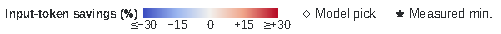
\includegraphics[width=\linewidth]{fig/experiments/fig08-cache-savings/fig08-cache-savings-color-key.pdf}\hfil}%
  \kern2bp
  \hbox to \linewidth{\hfil
    \subfigure[SW, Full]{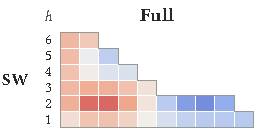
\includegraphics[width=.486\linewidth,trim=0bp 0bp 16bp 3.5bp,clip=false]{fig/experiments/fig08-cache-savings/fig08-cache-savings-a-sw-full.pdf}\label{fig:e4a-sw-full}}%
    \hspace{3.5bp}%
    \subfigure[SW, \textsf{LIMIT}~10]{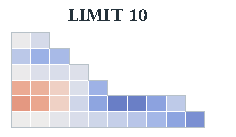
\includegraphics[width=.486\linewidth,trim=0bp 0bp 16bp 3.5bp,clip=false]{fig/experiments/fig08-cache-savings/fig08-cache-savings-c-sw-limit10.pdf}\label{fig:e4a-sw-topk}}%
    \hfil
  }%
  \kern3bp
  \hbox to \linewidth{\hfil
    \subfigure[LT, Full]{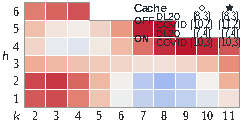
\includegraphics[width=.486\linewidth,trim=0bp 0bp 16bp 3.5bp,clip=false]{fig/experiments/fig08-cache-savings/fig08-cache-savings-b-lt-full.pdf}\label{fig:e4a-lt-full}}%
    \hspace{3.5bp}%
    \subfigure[LT, \textsf{LIMIT}~10]{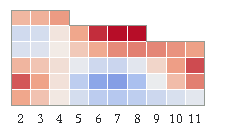
\includegraphics[width=.486\linewidth,trim=0bp 0bp 16bp 3.5bp,clip=false]{fig/experiments/fig08-cache-savings/fig08-cache-savings-d-lt-limit10.pdf}\label{fig:e4a-lt-topk}}%
    \hfil
  }%
}%
\endgroup
\par
\caption{Pooled input-token savings from prefix caching ($\beta{=}0$) on \DLtwozero{} and \COVIDshort{} at $n{=}500$ (illustrative $(k,h)$ insets).}
\label{fig:e4a-c2}
\end{figure}

% Standalone single-column vector trial from the existing synthetic fixture.
\begin{figure}[t]
  \centering
  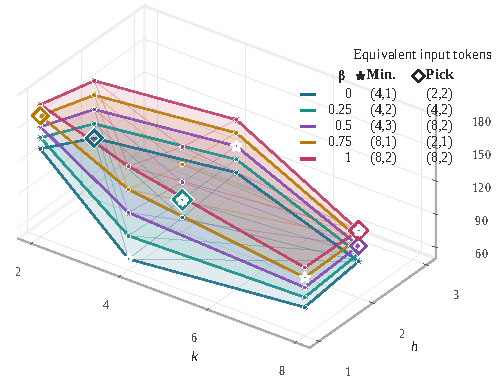
\includegraphics[width=\columnwidth]{fig/experiments/fig09-cache-discount/fig09-cache-discount-sensitivity.pdf}
  \caption{On-cold equivalent cost $C_\beta$ across five cache factors $\beta$. Stars mark empirical minima; diamonds mark planner picks.}
  \label{fig:e4b-beta}
\end{figure}

% The E4c scatter is omitted; its source and experimental records are retained.

\Needspace{327pt}
\subsection{Varying the Limit and Full Ranking}
\label{sec:exp:limit-sweep}
% Cost only: four independently rendered panels in a single-column 2x2 group; quality assets retained.
\begin{figure}[t]
\centering
\setlength{\subfigcapskip}{-1pt}\setlength{\subfigtopskip}{0pt}\setlength{\subfigbottomskip}{0pt}

\includegraphics[width=\columnwidth]{fig/experiments/fig10-limit-sweep/fig10-requested-k-cost-legend.pdf}\par
\vspace{1pt}
\subfigure[\fontsize{6.3bp}{7bp}\selectfont DL20, Off]{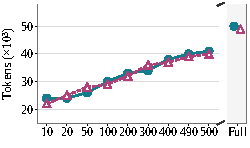
\includegraphics[width=.5\columnwidth]{fig/experiments/fig10-limit-sweep/fig10-requested-k-cost-a-dl20-off.pdf}}%
\subfigure[\fontsize{6.3bp}{7bp}\selectfont DL20, On-cold]{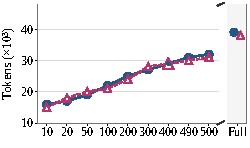
\includegraphics[width=.5\columnwidth]{fig/experiments/fig10-limit-sweep/fig10-requested-k-cost-b-dl20-on-cold.pdf}}\par\vspace{1pt}
\subfigure[\fontsize{6.3bp}{7bp}\selectfont COVID, Off]{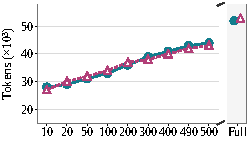
\includegraphics[width=.5\columnwidth]{fig/experiments/fig10-limit-sweep/fig10-requested-k-cost-c-covid-off.pdf}}%
\subfigure[\fontsize{6.3bp}{7bp}\selectfont COVID, On-cold]{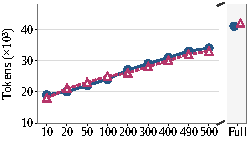
\includegraphics[width=.5\columnwidth]{fig/experiments/fig10-limit-sweep/fig10-requested-k-cost-d-covid-on-cold.pdf}}\par
{\fontsize{6.3bp}{7bp}\selectfont Requested $K$ (categorical); Full is separate}\par
\caption{Equivalent input-token cost across requested \LIMIT~$K$ prefixes and materialized Full ranking under cache Off and On-cold ($\beta{=}0$).}
\label{fig:e5-limit-sweep}
\end{figure}

\endgroup
